%Section1.tex

%%%%%%%%%%%%%%%%%%%%%%%%%%%%%%%%%%%%%%%%%%%%%%%%%%%%%%%%%%%%%%%%%%%%%%%%%%%%%%%%%%%%%%%%%%%%%%%%%%%%
\section{Real roots of univariate polynomials}\label{S:one}

Let $f\in\RR[x]$ be a polynomial.
It has the form
%
 \[
   f\ =\ c_kx^{a_k}  + \dotsb + c_{1}x^{a_{1}} + c_0x^{a_0}\,,
 \]
%
where $a_k> \dotsb > a_1 > a_0 \geq 0$ are integers and for $0\leq i \leq k$, $c_{i}\in\RR$ is nonzero.
Let $\defcolor{\var(c_0,\dotsc,c_k)}\vcentcolon=\#\{1\leq i\leq k\mid c_{i-1}c_i<0\}$ be the number of variations in sign of the
coefficients of $f$.
Descartes' Rule of Signs \cite{So_Book} gives an upper bound for the number of positive real roots of $f$.

%%%%%%%%%%%%%%%%%%%%%%%%%%%%%%%%%%%%%%%%%%%%%%%%%%%%%%%%%%%%%%%%%%%%%%%%%%%%%%%%%%%%%%%%%%%%%%%%%%%%
\begin{theorem}[Descartes' Rule of Signs]
  The number, $r$,  of positive real roots of $f$, counted with multiplicity, is at most $\var(c_0,\dotsc,c_k)$ and the difference
  $\var(c_0,\dotsc,c_k)-r$ is even.
\end{theorem}
%%%%%%%%%%%%%%%%%%%%%%%%%%%%%%%%%%%%%%%%%%%%%%%%%%%%%%%%%%%%%%%%%%%%%%%%%%%%%%%%%%%%%%%%%%%%%%%%%%%%

Given any sequence $c=(c_0,\dotsc,c_k)$, the \demph{variation}  \defcolor{$\var(c)$} of $c$ is the
number of variations in sign after removing all zero terms.
%
\begin{leftbar}
\verbatiminput{examples/variations.txt}
\end{leftbar}
%
For a sequence of polynomials  $\defcolor{f_\bullet}=(f_0,\dotsc,f_k)$ in $\RR[x]$ and $a\in\RR$, \defcolor{$\var(f_\bullet,a)$} is the
variation in the sequence 
$(f_0(a),\dotsc,f_{k}(a))$. 
We extend this to $a=\pm\infty$, by taking $f(\infty)$ to be the leading coefficient of $f(x)$ and $f(-\infty)$ to be the leading
coefficient of $f(-x)$.

Given a polynomial $f\in\RR[x]$ of degree $k$, consider its sequence of derivatives,
%
 \[
   \defcolor{\delta f}\ \vcentcolon= \left(f(x),f'(x),f''(x),\dots,f^{(k)}(x)\right)\,.
 \]
%
For $a<b$ in $\RR\cup\{\pm \infty\}$, let \defcolor{$r(f,a,b)$} be the number of roots of $f$ in the interval $(a,b\hspace{.05cm}]$, counted
with multiplicity.
Budan and Fourier~\cite[Ch.\ 2]{So_Book} generalized Descartes' Rule.

%%%%%%%%%%%%%%%%%%%%%%%%%%%%%%%%%%%%%%%%%%%%%%%%%%%%%%%%%%%%%%%%%%%%%%%%%%%%%%%%%%%%%%%%%%%%%%%%%%%%
\begin{theorem}[Budan-Fourier]
  We have that $r(f,a,b)\leq \var(\delta f,a) -\var(\delta f,b)$, and the difference
  $\var(\delta f,a) -\var(\delta f,b)-r(f,a,b)$ is even. 
\end{theorem}
%%%%%%%%%%%%%%%%%%%%%%%%%%%%%%%%%%%%%%%%%%%%%%%%%%%%%%%%%%%%%%%%%%%%%%%%%%%%%%%%%%%%%%%%%%%%%%%%%%%%

Descartes' Rule is when $a=0$ and $b=\infty$.
Let us consider an example.
%
\begin{leftbar}
\verbatiminput{examples/BudanFourierBound.txt}
\end{leftbar}
%
Note that $r(f,0,\infty)=r(f,-2,1)=3$.

In contrast to these bounds, 
Sylvester's Theorem determines the actual number of real roots, and more.
The \demph{Sylvester sequence}, \defcolor{$\Syl(f,g)$} of polynomials $f,g\in\RR[x]$ is the sequence
$\left(f_0,f_1,\dotsc,f_k\right)$ of nonzero polynomials, where $\defcolor{f_0}\vcentcolon= f$, $\defcolor{f_1}\vcentcolon= f'\cdot g$,
and for $i\geq 1$, 
%
  \[
    \defcolor{f_{i+1}}\ \vcentcolon=\ -1\cdot \mbox{remainder}(f_{i-1},f_i)\,,
  \]
%
the negative remainder term in the division of $f_{i-1}$ by $f_i$.
The last nonzero remainder is $f_k = \gcd(f,f'g)$.
Observe that for each $1\leq i\leq k$ there exists $\defcolor{q_i}\in\RR[x]$ such that
%
 \begin{equation}\label{Eq:divisionAlgorithm}
    f_{i-1}\ =\ q_i(x)f_i(x)-f_{i+1}(x)\,.
 \end{equation}
%
The \demph{reduced Sylvester sequence} $\defcolor{g_\bullet}=(g_0,\dotsc,g_k)$ is obtained by dividing each term in the Sylvester sequence
by $f_k=\gcd(f,f'g)$, so that $g_if_k=f_i$ for each $i$. 
Note that  $g_k=1$ and elements of the reduced Sylvester sequence satisfy~\eqref{Eq:divisionAlgorithm} with $f_j$ replacing $g_j$,


%%%%%%%%%%%%%%%%%%%%%%%%%%%%%%%%%%%%%%%%%%%%%%%%%%%%%%%%%%%%%%%%%%%%%%%%%%%%%%%%%%%%%%%%%%%%%%%%%%%%
\begin{theorem}[Sylvester]
  \label{Th:Sylvester}
  Let $f,g\in\RR[x]$ and suppose that $g_\bullet$ is the reduced Sylvester sequence of $f$ and $g$.
  For $a<b$ in $\RR\cup\{\pm\infty\}$ we have
  %
  \begin{eqnarray*}
    \qquad\var(g_\bullet,a)-\var(g_\bullet,b)&=&
    \#\{\zeta\in(a,b\hspace{.05cm}]\mid f(\zeta)=0\mbox{ and } g(\zeta)>0\}  \ -\
      \\
    && \#\{\zeta\in[\hspace{.05cm}a,b)\mid f(\zeta)=0\mbox{ and } g(\zeta)<0\}\,.\qquad
  \end{eqnarray*}
\end{theorem}
%%%%%%%%%%%%%%%%%%%%%%%%%%%%%%%%%%%%%%%%%%%%%%%%%%%%%%%%%%%%%%%%%%%%%%%%%%%%%%%%%%%%%%%%%%%%%%%%%%%%

Observe the different roles that the endpoints $\{a,b\}$ play in this formula.

%%%%%%%%%%%%%%%%%%%%%%%%%%%%%%%%%%%%%%%%%%%%%%%%%%%%%%%%%%%%%%%%%%%%%%%%%%%%%%%%%%%%%%%%%%%%%%%%%%%%
\begin{proof}
  In~\cite[Thm.\ 2.55]{BPR}, Sylvester's Theorem is stated and proven 
  when $f$ does not vanish at $a$ or at $b$, and it in terms of the Sylvester sequence $\Syl(f,g)$.
  That proof proceeds by studying $\var(\Syl(f,g), t)$ as $t$ increases fron $a$ to $b$, noting that it may only
  change when $t$ passes a root of some element of the Sylvester sequence.
  Since multiplying a sequence by a nonzero number $f_k(t)$ does not change its variation, the proof in~\cite{BPR} establishes this refined
  version when $f$ does not vanish at $a$ or at $b$.
  We proceed with the general case.

  The variation $\var(g_\bullet,t)$ may only change when $t$ passes a root $\zeta\in[a,b\hspace{.05cm}]$ of some $g_i$ in
  $g_\bullet$. 
  Observe that $\zeta$ cannot be a root of two consecutive elements of $g_\bullet$.
  If it were, then by~\eqref{Eq:divisionAlgorithm} and induction, it is a root of all elements of $g_\bullet$, and thus of
  $g_k=1$, which is a contradiction.
  Suppose that $g_i(\zeta)=0$ for some $i\geq 1$.
  By~\eqref{Eq:divisionAlgorithm} again, $g_{i-1}(x)$ and $g_{i+1}(x)$ have opposite signs for $x$ near $\zeta$ and thus
  $g_{i-1},g_i,g_{i+1}$ do not contribute to any change in $\var(g_\bullet,t)$ for $t$ near $\zeta$.
  This remains true if $\zeta=a$ and $t$ increases from $a$ or if $\zeta=b$ and $t$ approaches $b$.

  We now suppose that $g_0(\zeta)=0$ and thus $g_1(\zeta)\neq 0$.
  Then we have $f(\zeta)=0$.
  Let $m$ be the multiplicity of the root $\zeta$ of $f$ so that $f=(x{-}\zeta)^m h$ with $h(\zeta)\neq 0$.
  If $g(\zeta)=0$, then $(x{-}\zeta)^m$ divides $f'g$ and thus $f_k$, and so $g_0=f/f_k$ does not vanish at $\zeta$.
  Thus $g(\zeta)\neq 0$.

  Notice that $\defcolor{h_0}\vcentcolon=f/(x{-}\zeta)^{m-1}$ and $\defcolor{h_1}\vcentcolon=f'g/(x{-}\zeta)^{m-1}$ have the same signs for
  $x$ near $\zeta$ as do $g_0$ and $g_1$.
  A computation reveals that $h_1=mhg+(x{-}\zeta)h'g$.
 Choose $\epsilon>0$ so that $\zeta$ is the only root of any element in $g_\bullet$ lying in the interval
 $[\zeta-\epsilon,\zeta+\epsilon]$.
 We have
 %
 \[
 \begin{array}{c|c|l}
   x & h_0(x) & h_1(x)\\\hline
   \zeta-\epsilon & -\epsilon h(\zeta-\epsilon)  &
        mh(\zeta-\epsilon)g(\zeta-\epsilon) - \epsilon h'(\zeta-\epsilon)g(\zeta-\epsilon)  \rule{0pt}{13pt}\\
   \zeta     &     0    &   mh(\zeta)g(\zeta)  \rule{0pt}{13pt}\\
   \zeta+\epsilon & \epsilon h(\zeta-\epsilon)  &
        mh(\zeta+\epsilon)g(\zeta+\epsilon) + \epsilon h'(\zeta+\epsilon)g(\zeta+\epsilon)  \rule{0pt}{13pt}
 \end{array}
 \]
 %
 
 Suppose that $g(\zeta)>0$.
 Then the sign of $h_1$ on $[\zeta-\epsilon,\zeta+\epsilon]$ is opposite to the sign of $h_0(\zeta-\epsilon)$, but the same as the sign of
 $h_0(\zeta+\epsilon)$.
 Thus the variation $\var(g_\bullet,t)$ decreases by 1 as $t$ passes from $\zeta{-}\epsilon$ to $\zeta$, but is unchanged as $t$
 passes from $\zeta$ to $\zeta{+}\epsilon$.
  

 Suppose that $g(\zeta)<0$.
 Then the sign of $h_1$ on $[\zeta-\epsilon,\zeta+\epsilon]$ is the same as the sign of $h_0(\zeta-\epsilon)$, but opposite to the sign of
 $h_0(\zeta+\epsilon)$.
 Thus the variation $\var(g_\bullet,t)$ is unchanged as $t$ passes from $\zeta-\epsilon$ to $\zeta$, but increases by 1 as $t$ 
 passes from $\zeta$ to $\zeta+\epsilon$.

 Now consider the variation $\var(g_\bullet,t)$ for $t\in[a,b\hspace{.05cm}]$.
 This may only change at a number $\zeta\in[a,b]$ if $f(\zeta)=0$.
 If $g(\zeta)>0$ and $\zeta\neq b$, then it decreases by 1.
 If $g(\zeta)<0$ and $\zeta\neq a$, then it increases by 1.
 It is otherwise unchanged.
 This completes the proof.
 \end{proof}
%%%%%%%%%%%%%%%%%%%%%%%%%%%%%%%%%%%%%%%%%%%%%%%%%%%%%%%%%%%%%%%%%%%%%%%%%%%%%%%%%%%%%%%%%%%%%%%%%%%%

The \demph{Sturm sequence} of a polynomial $f\in\RR[x]$ is the Sylvester sequence $\Syl(f,1)$.
We may form the \demph{reduced Sturm sequence} as before.

%%%%%%%%%%%%%%%%%%%%%%%%%%%%%%%%%%%%%%%%%%%%%%%%%%%%%%%%%%%%%%%%%%%%%%%%%%%%%%%%%%%%%%%%%%%%%%%%%%%%
\begin{corollary}[Sturm's Theorem]
  Let $f\in\RR[x]$ and $a<b$ in $\mathbb{R}\cup\{\pm\infty\}$.
  Let $g_\bullet$ be the reduced Sturm sequence of $f$.
  Then the number of zeros of $f$ in the interval $(a,b\hspace{.05cm}]$ equals  $\var(g_\bullet,a) - \var(g_\bullet,b)$.
\end{corollary}
%%%%%%%%%%%%%%%%%%%%%%%%%%%%%%%%%%%%%%%%%%%%%%%%%%%%%%%%%%%%%%%%%%%%%%%%%%%%%%%%%%%%%%%%%%%%%%%%%%%%

Let us continue with the same polynomial $f=x(2x-3)(x^4-2)^2$ as before.
%
\begin{leftbar}
\verbatiminput{examples/Sturm.txt}
\end{leftbar}
%
Calling {\tt SturmCount(f)} without endpoints $a,b$ returns the total number of real roots of $f$.

Figure~\ref{F:One} shows the graph of $f$ in a neighborhood of its roots.
%%%%%%%%%%%%%%%%%%%%%%%%%%%%%%%%%%%%%%%%%%%%%%%%%%%%%%%%%%%%%%%%%%%%%%%%%%%%%%%%%%%%%%%%%%%%%%%%%%%%
\begin{figure}[htb]
  \centering
  \begin{picture}(220,125)

    \put(0,0){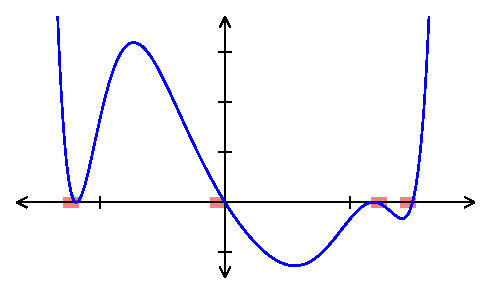
\includegraphics{pictures/graph_f}}
    \put(209,40){\small$x$}    \put( 90,114){\small$y$}
    \put( 31,24){\small$-1$}
    %\put(155,25){\small$1$}  \put(100, 9){\small$-3$}
    \put(105,57){\small$3$}  \put(105,81){\small$6$} \put(105,105){\small$9$}
        
  \end{picture}
\caption{Graph of $f$.}\label{F:One}
\end{figure}  
%%%%%%%%%%%%%%%%%%%%%%%%%%%%%%%%%%%%%%%%%%%%%%%%%%%%%%%%%%%%%%%%%%%%%%%%%%%%%%%%%%%%%%%%%%%%%%%%%%%%

An application of Sturm's Theorem is to give \demph{isolating intervals}, which are disjoint intervals each containing exactly one root
of $f$. 
Our implementation gives a list of pairs $\{p,q\}$ such that $(p,q]$ contains a unique root of $f$ and $q-p$ is less than a
user-provided tolerance.
The numbers $p,q$ are dyadic, lying in $\ZZ[\frac{1}{2}]$, as they are found in a binary search.
%
\begin{leftbar}
\verbatiminput{examples/realRootIsolation.txt}
\end{leftbar}
%
These isolating intervals are shaded in Figure~\ref{F:One}. 

Thomas~\cite{Thomas} observed that recursively iterating Sturm's Theorem on $f_k:=\gcd(f,f')$ can be used to give the number of real roots of
$f$, counted with multiplicity.
This same idea may be used to upgrade Sylvester's Theorem to give the count with multiplicity.
%
\begin{leftbar}
\verbatiminput{examples/SturmMultiplicity.txt}
\end{leftbar}
%

A polynomial $f\in\RR[x]$ is \demph{Hurwitz-stable} if its complex roots all have negative real parts.
Solutions to the system of constant coefficient ordinary differential equations 
%
 \[
  \dot{y}\ =\ Ay
 \]
%
are asymptotically stable ($\lim_{t\to\infty}y(t)=0$) when all eigenvalues $\zeta$ of $A$ have negative real part,
equivalently when the characteristic polynomial of $A$ is Hurwitz-stable.
 
Given a polynomial $f=c_kx^k+c_{k-1}x^{k-1}+\dotsb+c_0$,  let \defcolor{$H$} be the matrix
\[
\left(\begin{matrix}
  c_{k-1} & c_{k-3} & \dotsb & 0  & 0 \\
  c_k    & c_{k-2} &  \dotsb& 0 & 0 \\
  \vdots & \vdots & \ddots&    &\vdots\\
  \vdots & \vdots & & \ddots&\vdots\\
    0    &    0   & \dotsb&c_2 & c_0
\end{matrix}\right)
\]
For $1\leq \ell\leq k$, the \demph{Hurwitz determinant} \defcolor{$\Delta_\ell$} is the $\ell$th principal minor of $H$.


%%%%%%%%%%%%%%%%%%%%%%%%%%%%%%%%%%%%%%%%%%%%%%%%%%%%%%%%%%%%%%%%%%%%%%%%%%%%%%%%%%%%%%%%%%%%%%%%%%%%
%Hurwitz stability
\begin{theorem}[Hurwitz~\cite{Hurwitz}]
  Suppose that $c_k>0$.
  Then $f$ is Hurwitz-stable if and only if all the Hurwitz determinants $\Delta_{1},\dots,\Delta_{k}$ are positive.
\end{theorem}
%%%%%%%%%%%%%%%%%%%%%%%%%%%%%%%%%%%%%%%%%%%%%%%%%%%%%%%%%%%%%%%%%%%%%%%%%%%%%%%%%%%%%%%%%%%%%%%%%%%%

{\tt Realroots} implements both the Hurwitz matrix and this test for Hurwitz-stability.
%
\begin{leftbar}
\verbatiminput{examples/Hurwitz.txt}
\end{leftbar}
%
